
%(BEGIN_QUESTION)
% Copyright 2008, Tony R. Kuphaldt, released under the Creative Commons Attribution License (v 1.0)
% This means you may do almost anything with this work of mine, so long as you give me proper credit

Calculate all voltage drops and currents in this circuit, complete with arrows for current direction and polarity markings for voltage polarity.  Then, calculate the overall voltage gain of this amplifier circuit ($A_V$), both as a ratio and as a figure in units of decibels (dB):

$$\includegraphics[width=15.5cm]{i03261x01.eps}$$

\vskip 20pt \vbox{\hrule \hbox{\strut \vrule{} {\bf Suggestions for Socratic discussion} \vrule} \hrule}

\begin{itemize}
\item{} Identify the ``simplifying assumptions'' we generally use when analyzing DC opamp circuits.  Hint: one has to do with the effect of negative feedback on the input voltages, and another has to do with the input terminal currents.
\item{} Explain how this circuit would respond if the 10 k$\Omega$ resistor failed open.
\item{} Explain how this circuit would respond if the 10 k$\Omega$ resistor failed shorted.
\item{} Explain how this circuit would respond if the 2.7 k$\Omega$ resistor failed open.
\item{} Explain how this circuit would respond if the 2.7 k$\Omega$ resistor failed shorted.
\item{} Explain how this circuit would respond if the (+) and ($-$) opamp inputs were swapped.
\end{itemize}

\underbar{file i03261}
%(END_QUESTION)





%(BEGIN_ANSWER)

$$\includegraphics[width=15.5cm]{i03261x02.eps}$$

$A_V$ = 4.704 = 13.449 dB

\vskip 10pt

Follow-up question: how much input impedance does the $-2.35$ volt source ``see'' as it drives this amplifier circuit?

%(END_ANSWER)





%(BEGIN_NOTES)

Operational amplifier circuits provide a great opportunity to review basic concepts of DC circuits: voltage drops, polarity, current directions, Ohm's Law, Kirchhoff's Voltage Law, Kirchhoff's Current Law, etc.  This circuit is no exception.  Emphasize the fact that a great many opamp circuits may be comprehensively analyzed merely with knowledge of these fundamental principles and the characteristics of an ideal opamp (zero input current, infinite open-loop gain, unlimited output voltage swing, zero voltage between input terminals when negative feedback is in effect).

The follow-up question is important because it showcases one of the great advantages of using noninverting opamp amplifier circuits as voltage signal amplifiers: extremely high input impedance.  This would be a good opportunity to review typical input impedance values for operational amplifiers, by showing datasheets for some typical opamps and for some non-typical (i.e. MOSFET input) opamps.

%INDEX% Electronics review: opamp noninverting amplifier circuit

%(END_NOTES)


